%% =============================================================================
%%  fig_filter_col.tex -- the snoop filter's decision path, single-column
%%  version of fig_filter.tex for the paper.
%%
%%  Build:  pdflatex fig_filter_col.tex   ->  fig_filter_col.pdf
%%
%%  Same content and the same routing rules as fig_filter.tex (see its header),
%%  folded to 89 mm: the request is labelled at the bus start instead of a
%%  source box, PE 1-3 collapse into one block whose three outputs run straight
%%  down, and the NOR sits left of the arbiter box rather than above it.
%%  After rotate=-90, "input 2" of a two-input gate is the LEFT input; on the
%%  four-input NOR, input 4 is leftmost. Sources further right take lower jogs.
%% =============================================================================
\documentclass[border=2pt]{standalone}
\usepackage{tikz}
\usepackage{times}
\usepackage{amssymb}
\usetikzlibrary{arrows.meta,calc,shapes.gates.logic.US}

\begin{document}
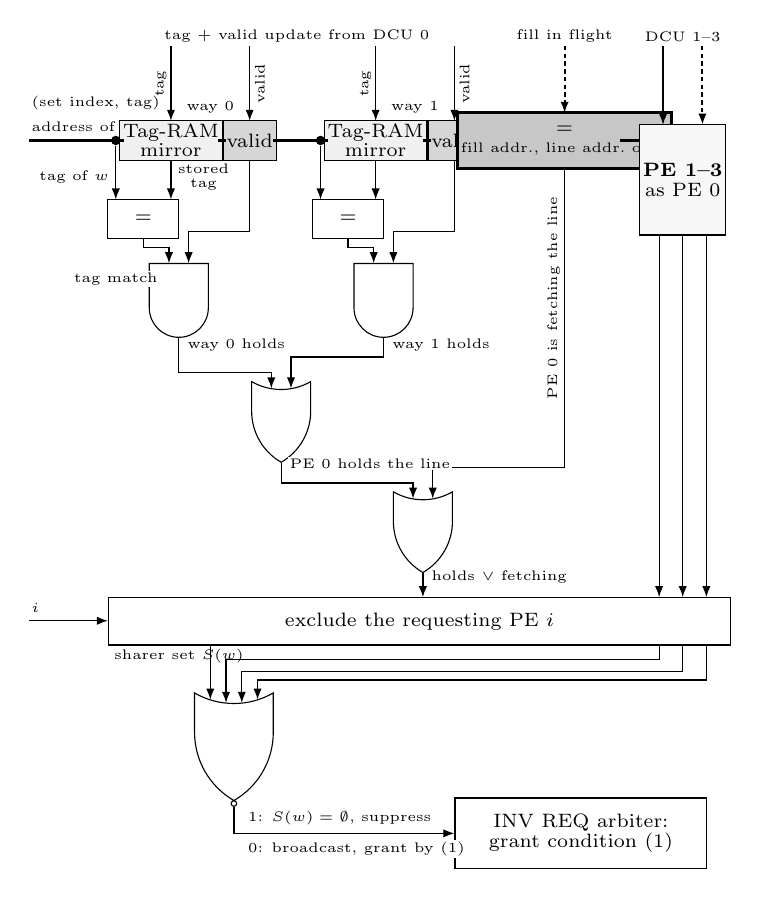
\begin{tikzpicture}[
  x=1mm, y=1mm, font=\scriptsize,
  box/.style  ={draw,rectangle,align=center,inner sep=1.2pt},
  ram/.style  ={box,fill=black!6},
  ff/.style   ={box,fill=black!16},
  op/.style   ={box,fill=white},
  pe/.style   ={box,fill=black!3},
  new/.style  ={box,fill=black!22,line width=1.1pt},
  g2/.style   ={draw,logic gate inputs=nn,logic gate input sep=5mm,rotate=-90,scale=0.5},
  g4/.style   ={draw,logic gate inputs=nnnn,logic gate input sep=4mm,rotate=-90,scale=0.5},
  ln/.style   ={draw,-{Latex[length=1.4mm]},line width=0.45pt},
  bus/.style  ={draw,line width=1.1pt},
  mir/.style  ={draw,-{Latex[length=1.4mm]},dashed,dash pattern=on 1.6pt off 1.2pt,line width=0.7pt},
  dot/.style  ={circle,fill=black,inner sep=0,minimum size=1.2mm},
  lab/.style  ={font=\tiny,inner sep=0.7pt,fill=white,align=center},
  labr/.style ={font=\tiny,inner sep=0.4pt,rotate=90,anchor=center},
]

% ----------------------------------------------------------- the address bus
\draw[bus] (0, 0) -- (10, 0);
\node[lab,anchor=south west] at (0, 0.8) {address of $w$};
\node[lab,anchor=south west] at (0, 3.6) {(set index, tag)};

% ----------------------------------------------------------- PE 0 in full
\node[lab,anchor=south] at (34, 12.2) {tag + valid update from DCU 0};
\node[lab,anchor=south] at (68, 12.2) {fill in flight};

% two ways, centres c = 17 and 43
\foreach \k/\c in {0/21, 1/47} {
  \node[dot] (tp\k) at (\c-10, 0) {};
  \node[ram,minimum width=12mm,minimum height=5mm] (tr\k) at (\c-3, 0)
    {Tag-RAM\\[-1pt]mirror};
  \node[ff,minimum width=6mm,minimum height=5mm] (vb\k) at (\c+7, 0) {valid};
  \draw[bus] (\c-11, 0) -- (\c-9, 0);
  \draw[bus] (\c+3, 0) -- (\c+4, 0);
  \draw[bus] (\c+10, 0) -- (\c+16, 0);
  \draw[ln] (\c-3, 12) -- (\c-3, 2.5);
  \draw[ln] (\c+7, 12) -- (\c+7, 2.5);
  \node[labr] at (\c-4.3, 7.2) {tag};
  \node[labr] at (\c+8.3, 7.2) {valid};
  \node[lab] at (\c+2, 4.2) {way \k};
  \node[op,minimum width=9mm,minimum height=5mm] (cp\k) at (\c-6.5, -10) {$=$};
  \draw[ln] (tp\k) -- (\c-10, -7.5);
  \draw[ln] (tr\k.south) -- (\c-3, -7.5);
  \node[and gate US,g2] (an\k) at (\c-2, -20) {};
  \draw[ln] (cp\k.south) |- ($(an\k.input 2)+(0,2)$) -- (an\k.input 2);
  \draw[ln] (vb\k.south) |- ($(an\k.input 1)+(0,4)$) -- (an\k.input 1);
}
\node[lab,anchor=east] at (10.4, -4.6) {tag of $w$};
\node[lab,anchor=west] at (18.6, -4.6) {stored\\[-1pt]tag};
\node[lab,anchor=east] at (16.6, -17.6) {tag match};

% fill comparator, also on the bus
\node[new,minimum width=14mm,minimum height=7mm] (fc0) at (68, 0)
  {$=$\\[-1pt] {\tiny fill addr., line addr.\ of $w$}};
\draw[mir] (68, 12) -- (68, 3.5);
\draw[bus] (75, 0) -- (78, 0);

% OR over the two ways, then OR with the fill term
\node[or gate US,g2] (orw) at (32, -35) {};
\draw[ln] (an0.output) |- ($(orw.input 2)+(0,2)$) -- (orw.input 2);
\draw[ln] (an1.output) |- ($(orw.input 1)+(0,4)$) -- (orw.input 1);
\node[lab,anchor=west] at (19.8, -26) {way 0 holds};
\node[lab,anchor=west] at (45.8, -26) {way 1 holds};
\node[or gate US,g2] (orf) at (50, -49) {};
\draw[ln] (orw.output) |- ($(orf.input 2)+(0,2)$) -- (orf.input 2);
\draw[ln] (fc0.south) |- ($(orf.input 1)+(0,4)$) -- (orf.input 1);
\node[lab,anchor=west] at (32.8, -41) {PE 0 holds the line};
\node[labr] at (66.6, -20) {PE 0 is fetching the line};
\draw[ln] (orf.output) -- (50, -58);
\node[lab,anchor=west] at (50.8, -55.5) {holds $\vee$ fetching};

% ----------------------------------------------------------- PE 1..3 collapsed
\node[pe,minimum width=10mm,minimum height=14mm] (blk) at (83, -5)
  {\textbf{PE 1--3}\\[-1pt] as PE 0};
\draw[ln]  (80.5, 12) -- (80.5, 2);
\draw[mir] (85.5, 12) -- (85.5, 2);
\node[lab,anchor=south] at (83, 12.2) {DCU 1--3};
\foreach \x in {80, 83, 86} { \draw[ln] (\x, -12) -- (\x, -58); }

% ----------------------------------------------------------- sharer set
\node[op,minimum width=79mm,minimum height=6mm,anchor=north west] (mask) at (10, -58)
  {exclude the requesting PE $i$};
\draw[ln] (0, -61) -- (10, -61);
\node[lab,anchor=south west] at (0, -60.3) {$i$};
\node[lab,anchor=north west] at (10.5, -64.3) {sharer set $S(w)$};

% NOR over the four bits of S(w); sources further right take lower jogs
\node[nor gate US,g4] (nor) at (26, -76) {};
\draw[ln] (50, -64) |- ($(nor.input 4)+(0,7)$)   -- (nor.input 4);
\draw[ln] (80, -64) |- ($(nor.input 3)+(0,5.5)$) -- (nor.input 3);
\draw[ln] (83, -64) |- ($(nor.input 2)+(0,4)$)   -- (nor.input 2);
\draw[ln] (86, -64) |- ($(nor.input 1)+(0,2.5)$) -- (nor.input 1);

\node[op,minimum width=32mm,minimum height=9mm,anchor=west] (arb) at (54, -88)
  {INV REQ arbiter:\\[-1pt] grant condition (1)};
\draw[ln] (nor.output) |- (54, -88);
\node[lab,anchor=south west] at (27.5, -87.2) {1: $S(w)=\emptyset$, suppress};
\node[lab,anchor=north west] at (27.5, -88.8) {0: broadcast, grant by (1)};

\end{tikzpicture}
\end{document}
